\section{资源势垒：功率通量、结合能与物质丰度}

智能在表示空间中把路径选出来之后，代价要在介质里结算，而介质的第一道账就是资源账。三类约束中，资源势垒最容易被误判。讨论智能的能力时，限制条件通常被设在信息一侧：模型够不够强，数据够不够多，算法够不够好，这些条件确实在快速改善，改善的幅度也可以测量。但一个方案要从描述变成事实，还要通过另一套判据完全不同的检查：材料能否取得，能量能否以需要的功率注入，过程能否在可接受的时间内完成，形成的结构能否被长期维持。物质世界不会因为一个方案被提出就自动改变。图纸可以瞬间生成，路线可以快速优化，模型可以在屏幕上推演无数可能，但只要一个方案要进入现实，它就必须回答更古老的问题：材料从哪里来，能量如何注入，过程如何展开，结构如何稳定，损耗如何处理，秩序如何维持。这就是资源势垒。

资源势垒不是简单的“缺资源”，也不是某种暂时性的供应不足，而是任何物质重构都必须穿过的状态转移条件。现实系统从状态A变成状态B，不是符号排列的变化，而是物质位置、能量分布、结构关系和时间过程的重新配置。信息可以提供配方，智能可以选择路径，组织可以协调行动，但物质本身不会因为算法更优而自动重排。资源也不是自然界中孤立存在的“东西”：它不是元素表上的名称，也不是地壳里的总储量，而是物质处在可提取、可分离、可加工、可运输、可控制、可维护的状态中。资源不是原子本身，而是物质、可用能、位置、结构、纯度、接口和可用性的组合。没有可用状态，存在不等于资源；没有进入技术系统的通道，储量不等于能力。所以，资源势垒的第一性问题不是“有没有”，而是“能不能把它带入可用状态”。

铁、硅、氮、锂、铜、铝都可以在自然中找到，但自然存在并不自动等于技术可用。物质要进入技术系统，必须经过提取、分离、提纯、运输、加工、稳定和维护。每一步都需要可用能，每一步都会产生损耗，每一步都要依赖设备、组织和时间。可用性因此不是物质的属性，而是技术系统的工作结果，这一点反过来解释了为什么同一片土地在不同技术水平下承载的人口和产业相差极大，也解释了为什么资源统计总是滞后于技术能力的变化。所谓资源，是技术系统在自然物质中制造出来的可用性。

\subsection{功率通量限制与卡尔达肖夫标度}

\subhead{可用能的能级}

这里的“可用能约束”不是把某一种热力学势函数直接套用于所有技术系统，而是泛指能够推动状态转移、维持局部有序并被技术系统实际调用的能量条件。对一个工程系统来说，关键不只是能量总量，而是能量能否以合适的形式、功率、位置、时间窗口和控制精度进入过程。热量、燃料、电力、机械功、化学势和位势都可能参与现实改变，但它们只有在可被技术系统调度、转换和约束时，才真正成为能力。可用能的形式也不止一种：城市和基础设施把大量材料抬升、固定、连接起来，本质上是把可用能以重力位势的形式存入结构，这笔势能只有在拆除和搬运时才会被重新取出，浓度、位置和纯度与能量一样构成状态转移的前置条件。

那么，一种可用能究竟能支撑起多大的重构能力，这一点取决于它处在哪一个能级上。1964年，卡尔达肖夫提出用文明能够支配的功率来划分文明等级\cite{kardashev1964transmission}，该标度通常写成
\begin{equation}
K=\frac{\log_{10}P-6}{10},
\label{eq:kardashev}
\end{equation}
这里$K$为文明等级，无量纲；$P$为该文明能够支配的总功率，单位瓦特；分母10的含义是指数每变化0.1，对应功率提高1个数量级，$K$每增加1，对应功率提高10个数量级。按这个标度，1级对应$10^{16}$瓦；人类目前的功率消耗大约在$2\times10^{13}$瓦量级，即20太瓦，代入得$K\approx0.73$，与1.0之间相差约2.7个数量级。\cite{smil2017energy}文献中常引用的另一种口径把地球接收到的全部太阳辐射（约$1.7\times10^{17}$瓦）算作1级，按本式它对应$K\approx1.12$；两种口径的差别只是零点不同，不影响下面的结论。在这个坐标系里，0.73与1.0之间不是27\%的差距。

化学反应与核反应具有不同的单次能量尺度，核裂变已经是现实电力来源，太阳能、水电与风电也不以人类燃烧化学燃料为前提。\cite{jaffe2018physics} 能量来源的微观尺度，不能直接决定一座工厂可获得的宏观功率。工业过程还受能量转换、输送、设备、材料和控制条件约束。

不过，这个标度容易被误读成一条单维排名。功率总量只是文明能力的一个坐标，同样的功率，以什么形式、在什么位置、用多高的控制精度释放，结果差别很大；反过来，一个功率总量不高但调度能力很强的系统，可以在特定领域完成功率更大的系统做不到的状态转移。卡尔达肖夫指数回答的是上限问题，不是全部问题，把$K$值当成文明评分，会漏掉可用能形式、释放位置和控制窗口这三个变量。

从这个角度看，技术的第一性对象不是信息，而是由物质、能量和约束共同维持的局部有序结构。桥梁、芯片、电池、药物、工厂、城市、数据中心，都不是单纯的“物体”。它们是物质被能量推离分散、无序或不可用状态之后形成的功能结构。它们要被制造出来，要在扰动中保持功能，还要不断对抗磨损、腐蚀、热、噪声、老化和故障。技术不是把想法变成现实这么简单，而是把可用能转化为可控、稳定、可维护的局部秩序，热力学和能源史反复说明，文明不是脱离能量的符号系统，而是依赖能量转换、物质组织和废热排出的开放过程。\cite{smil2017energy,callen1985thermodynamics}

\subhead{化学能之上的台阶}

核裂变通过核燃料、反应堆与热力循环提供功率，同时带来燃料供给、材料、废物与安全治理要求。它能否长期扩大使用，要比较资源路线、技术、成本和制度条件，不能仅由天然铀235丰度或废物存在直接判定。化学、核与其他能源各自的约束，应在完整系统上核算。

氘氚聚变单次释放约17.6兆电子伏特。实现有用净能量还需要满足等离子体约束、材料、氚循环、排热和设备运行条件。\cite{atzeni2004physics} 聚变若形成成熟能源系统，可能扩大供给选择；在此之前，工业能力仍可通过现有能源、转换与工艺继续改进，并不被统一锁在一种价电子能级上。

火箭方程显示，给定有效排气速度时，较大的速度增量需要迅速上升的质量比。化学推进具有实际性能范围，约每秒4.5公里是高性能化学发动机的代表量级，并非所有设计共享的严格上限。任务还可采用分级、引力辅助或其他推进方式。约束的力量在于可以逐项计算，而不是直接从单次反应能量宣布活动半径。

\begin{equation}
\Delta v=v_{e}\,\ln\frac{m_{0}}{m_{f}},
\qquad
\frac{m_{0}}{m_{f}}=\exp\!\left(\frac{\Delta v}{v_{e}}\right)
\end{equation}

式中 $\Delta v$ 为火箭获得的速度增量，单位米每秒；$v_{e}$ 为有效排气速度，单位米每秒，它的上限由反应热给出，正文给出的量级是每秒 4.5 公里；$m_{0}$ 为起飞质量，$m_{f}$ 为推进剂耗尽之后的质量，单位千克；两者之比称为质量比，无量纲。对数是这个式子的全部要害：速度增量每增加一个 $v_{e}$，质量比就乘一次 $e$，想要的速度增量越大，必须留给燃料的质量比例越高，而 $v_{e}$ 的上限由化学键能级设定，所以这不是发动机设计的问题。正文所说“绝大部分起飞质量必须留给燃料、人类的活动半径因此被锁在地球附近”，写出来就是质量比随 $\Delta v/v_{e}$ 指数上升。它的适用边界是：这里给出的是理想速度增量，忽略空气阻力与重力损失，真实任务所需的推进剂比它算出的更多；本书不代入具体任务的目标 $\Delta v$，因为那取决于任务本身，这个式子在这里的作用只是说明 $v_{e}$ 的量级如何限定宏观迁移成本。

\subhead{计算速率与功率速率的失配}

计算、储能与执行器的改进路径不同。电池的比能量、比功率、寿命、安全与成本要同时权衡；电芯、包级系统与理论材料值也须分开。比较燃料与电池，还要计入发动机和电机效率及任务质量。历史年改善率不是永恒常数，按百分比复合增长也不是线性增长。\cite{ziegler2021reexamining,viswanathan2022challenges}

布雷默曼与贝肯斯坦一类理论界限，分别讨论特定假设下的信息处理或信息容量。\cite{bremermann1982minimum,bekenstein1981universal} 它们不能用来推算商用芯片还有多少年可按当前速度改进。设备的可用进步还受材料、互连、存储、散热和制造经济性限制；机器人行动则要另算执行器与储能的功率账。

\subhead{四组条件}

把技术看作局部有序结构的生成过程，物质重构要穿过的条件就可以逐项列出。第一组是材料条件：现实改变需要载体，桥梁需要钢材和混凝土，电池需要金属、隔膜和电解质，芯片需要高纯材料，药物需要可合成、可稳定、可进入身体的分子。没有载体，信息只是描述；载体不合适，方案就无法进入世界。很多技术不是败给想象力，而是败给材料形态、纯度、技术链条、寿命和长期稳定性。第二组是可用能条件：材料从一种状态进入另一种状态，通常要跨越势垒，矿石要还原，分子键要断裂，晶格要重组，物体要搬运，结构要抬升，设备要驱动。能量不是附加因素，而是状态转移的条件，没有足够可调用、可控制、可集中释放的可用能，物质不会因为人类更聪明就自动形成新的秩序，经济过程中的生产、转化和废弃，也不能脱离熵增、耗散和不可逆性。\cite{georgescu1971entropy}

第三组是过程条件，它的特点是过程的速度对温度高度敏感。现实改变不是瞬间发生的，钢铁要冶炼，水泥要煅烧，药物要合成和验证，芯片要经历多道工艺，建筑要施工、养护、检查和交付；过程需要设备、时序、环境、人员和稳定条件，许多物理过程不能像软件一样复制、回滚或重启，过程越精密，对温度、压力、纯度、时机和环境的要求越苛刻。这种敏感性有确定的物理形式，反应速率与温度之间的关系由阿伦尼乌斯关系描述，它的表达式和适用条件在处理强共价键断裂时给出。这里先记住它的结论：活化能越高，温度对速率的影响越剧烈，温度在高温工艺里不是线性放大器，而是越过势垒的开关。

第四组是维持条件，它把前三组的账目从一次性投入变成长周期支出。一个有序结构不是建成之后就永久存在，机器会磨损，建筑会老化，管道会腐蚀，材料会疲劳，数据中心要冷却，基础设施要维护，药物体系要监管，局部有序结构不是一次性成果，而是持续抵抗耗散的状态，维持秩序本身，就是资源势垒的一部分。这四组条件构成了物质重构的底层关系：信息提供配方，材料提供载体，可用能完成做功，过程展开结构，维持机制抵抗耗散。这个关系里没有任何一项可以被信息完全替代，只有配方，没有载体，结果不会出现；只有载体，没有可用能，状态不会改变；只有能量，没有过程，结构不会稳定；只有局部有序，没有持续维护，系统无法长期存在。

这四组条件的清单容易被读成一张审批表，似乎逐项通过就能进入现实。实际的情形不是这样，四项必须同时在场，任何一项接近于零，其余三项的投入都无法结算：材料短缺会让可用能空转，可用能不足会让过程停在半途，过程失控会让维持成本超过结构本身的价值。资源势垒的核心含义正在这里：\key{现实不是由可能性组成，而是由可执行状态组成。}可能性可以无限生成，可执行状态必须满足物质条件。一个方案成立，不等于材料已经到位；材料存在，不等于可用能已经注入；能量足够，不等于过程已经稳定；过程完成，不等于结构可以长期维持，真正的现实改变，必须穿过从材料到可用能、从工艺到维护、从局部状态到长期秩序的完整链条。

这四组条件在历史的每个阶段并不以同样的强度生效。技术系统曾经长期绕开其中最昂贵的一项：它并不自己制造所需的低熵结构，而是直接取用自然过程已经完成的产物。木材有强度，纤维有韧性，河流有落差，煤炭有化学能，在那种起点上，材料条件、过程条件和维持条件的账目要轻得多。取用自然预制结构的代价，是把技术系统的规模上限交给了自然过程的产出速率；一旦需求超过这个速率，四组条件就会同时以完整强度回到账面上。这种取用能持续多久，决定了资源势垒此后以什么样的形式重新出现。

\subsection{低活化能物质利用与物理形态重构}

技术史的起点不是制造物质，而是挑选物质。人类最早使用的材料和动力，几乎都不是自己合成的，它们是被光合作用、地质过程和演化过程提前制造好的结构。理解这种取用的性质，才能理解早期技术为什么显得轻巧，以及这种轻巧为什么不可持续。

最早的技术，并不是制造世界，而是利用世界已经制造好的部分。木材、棉花、兽皮、骨骼、水流、风力、动物肌肉、煤炭和石油，都不是人类从零创造的资源。它们是自然过程已经组织好的结构，或者已经积累好的能量形态。树木把阳光、二氧化碳和水转化成纤维，植物和动物把环境中的物质组织成身体，河流和风场把能量流排列成方向，化石燃料把远古生命捕获的太阳能封存在化学键中。早期技术之所以显得轻巧，不是因为它摆脱了物理，而是因为它调用了自然已经完成的工作，这就是低垂果实的真正含义。

\subhead{自然预制结构的取用}

低垂不是低级，而是自然已经预付了一部分账单。人不需要自己合成木材，不需要自己设计棉纤维，不需要自己即时制造煤炭中的化学能，自然已经替技术系统预付了能量、结构和时间，技术只是在这些预制结构上切割、搬运、编织、燃烧、驯化和重排。换言之，低垂果实不是容易的果实，而是自然已经完成低熵结构生成的地方。木头已有强度，石头已有硬度，纤维已有韧性，肌肉已有机械功，河流已有落差，煤炭已有化学能，早期技术沿着自然给出的低阻路径前进，它主要改变形态，而不是重写物质本身；主要调用已有秩序，而不是从无序中制造秩序。这也解释了为什么很多早期技术看起来格外“自然”：风车不是制造风，而是拦截风；水车不是制造落差，而是利用落差；木屋不是制造纤维素结构，而是切割树木；驯化动物不是制造肌肉，而是组织动物已有的代谢和运动能力。技术并不是没有成本，而是大量成本已经被地质、生命和气候过程提前摊销。

棉花把自然形成的纤维素结构带入纺织加工。植物已完成材料合成，纺织机械主要组织牵伸、加捻与卷绕。\cite{klemm2005cellulose} 这一形态适配是机械化的重要条件，工业革命的发生还涉及能源、贸易、资本、劳动与制度，不能由“当时没有断开强化学键的能量密度”单独解释。

能适应早期粗糙机械加工的，不只有化学上的低活化能，还有微观形态上的适配。棉纤维沿轴向分布着天然转曲，这不是随机缺陷，而是细胞壁在脱水过程中因层积差异形成的螺旋状扭曲：棉铃成熟开裂、水分蒸发之后，原本圆柱形的细胞塌陷，形成带物理咬合点的三维形态。纤维之间的摩擦因此被显著放大，纺纱机只需施加较小的加捻力矩，就能在纤维间产生很大的法向压力，把松散的短纤维抱合成连续纱线。羊毛表面有鳞片，摩擦系数不小却容易毡化纠缠，难以适应高速机械梳理；亚麻表面平直光滑，抱合力差，必须借助高能耗的湿纺。棉花正好落在无需化学粘合、仅靠机械力学就能完成重构的区间，所以早期纺纱机可以用极低的功率驱动。标准化是另一半原因。羊毛受个体差异、生长部位和环境波动影响，直径、长度和卷曲度都呈离散分布，处理这种原料需要人的手和眼进行实时反馈，这超出了刚性机械的能力。棉花是种子纤维，细度、长度和成熟度受基因表达和种植条件严格约束，方差很小。水力纺纱机不需要视觉识别，也不需要触觉反馈，它只需要重复执行牵伸、加捻、卷绕这套固定动作，因为输入端的变异已经被生物学规律限制在可控范围内。

但低垂果实不会无限延伸。随着需求扩大，技术系统不再满足于自然给出的形态：木材不够坚硬，需要钢铁；天然肥力不够稳定，需要化肥；自然纤维不够多样，需要合成材料；自然晶体不够精密，需要半导体；普通燃烧不够可控，需要电力系统；自然药物不够精确，需要合成分子和靶向干预。技术开始从调用已有结构，转向主动制造结构。

\subhead{活化能阶梯}

从调用已有形态转向主动制造，工艺条件通常更复杂。本书把这种变化称为“活化能阶梯”，指向提纯、反应、晶格、缺陷与界面控制等门槛。各工艺的活化能具有明确物理含义，整座工厂的资本和维护负担则没有一个统一的活化能数值。二者需要分开测量。

技术可用性取决于材料是否达到需要的纯度、形态、浓度与位置。沙子不是晶圆，矿石不是钢材，地层中的锂也不是电池。形成可用状态需要提取、运输、加工、反应与质量控制，其成本既包括热力学和动力学条件，也包括设备与组织。

精密制造常需要更严格的洁净、缺陷、测量与过程窗口。芯片缩小以后，某些控制任务会更难，同时也可能通过工艺创新降低单位功能成本。需要核算的是具体步骤的能耗、良率、资本与维护，不能把所有控制难度都归入一个逐级升高的活化能。

启动与维持应放进同一生命周期。更精细的结构可能增加控制与维护要求，也可能以更少材料、更低能耗完成同一功能。技术深入物质底层，并不保证总成本单向上升；它要求核算从发现、制造到长期运行的完整路径。
\begin{figure}[ht]
\centering
% >>>>>>>>>> figs/fig-activation-ladder.tex >>>>>>>>>>
% 图 2-1  活化能阶梯与供给上限
% 纵轴为对数能标（1 个数量级 = 0.48 cm），左右同尺度。
% 四根柱子是四档重构任务的「需求」，越高越难做；
% 三条虚线是三类能源的「供给上限」。阴影带是智能真正够得着的区间。
% 读图要点：第三档（强键断裂）恰好顶在化学能上限上——合成氨、炼铁之所以
% 昂贵，不是因为工艺不巧，而是因为要断的键与能支付的能处在同一量级。
\begin{tikzpicture}[x=1cm, y=1cm, font=\small,
  ax/.style={-{Stealth[length=2.0mm]}, ink, line width=0.6pt},
  ytick/.style={anchor=east, font=\scriptsize, text=slate},
  upln/.style={line width=0.75pt, dashed}
]
\useasboundingbox (-0.55,0.80) rectangle (11.85,-7.10);

\def\aX{1.05} \def\aY{-5.10} \def\u{0.48} \def\aR{11.20}
\pgfmathsetmacro{\yTop}{\aY+\u*9.5}

% ---------- 坐标轴 ----------
\draw[ax] (\aX,\aY) -- (\aR,\aY);
\draw[ax] (\aX,\aY) -- (\aX,\yTop)
      node[anchor=south, font=\scriptsize, text=ink, yshift=1pt] {单位活化能 (kJ/mol)};
\foreach \e/\t in {0/1,2/{100},4/{$10^{4}$},6/{$10^{6}$},8/{$10^{8}$}} {
  \pgfmathsetmacro\yy{\aY+\u*\e}
  \draw[slate!55, line width=0.4pt] (\aX,\yy) -- ({\aX-0.07},\yy);
  \node[ytick] at ({\aX-0.09},\yy) {\t};
}

% ---------- 智能可改动区间（先铺底，柱压其上）----------
\fill[forest!11] ({\aX+0.03},{\aY+\u*1.00}) rectangle ({\aR-0.05},{\aY+\u*3.00});

% ---------- 四档需求 ----------
\def\bw{0.90}
\foreach \cx/\hi/\col in {2.00/1.30/terra, 3.90/1.80/terra, 5.80/3.00/deepblue, 7.70/9.00/rust} {
  \pgfmathsetmacro\yt{\aY+\u*\hi}
  \fill[\col!20] ({\cx-\bw/2},{\aY+0.02}) rectangle ({\cx+\bw/2},\yt);
  \draw[\col!80, line width=0.9pt] ({\cx-\bw/2},{\aY+0.02}) rectangle ({\cx+\bw/2},\yt);
  \draw[\col!90, line width=2.4pt] ({\cx-\bw/2},\yt) -- ({\cx+\bw/2},\yt);
}
\node[font=\scriptsize, text=ink, anchor=north, align=center] at (2.00,-5.22) {取用预制结构};
\node[font=\scriptsize, text=ink, anchor=north, align=center] at (3.90,-5.22) {弱键重排};
\node[font=\scriptsize, text=ink, anchor=north, align=center] at (5.80,-5.22) {强键断裂};
\node[font=\scriptsize, text=ink, anchor=north, align=center] at (7.70,-5.22) {核反应};
\node[font=\scriptsize, text=slate, anchor=north, align=center] at (2.00,-5.92) {选矿、溶解};
\node[font=\scriptsize, text=slate, anchor=north, align=center] at (3.90,-5.92) {氢键 $\sim$20};
\node[font=\scriptsize, text=slate, anchor=north, align=center] at (5.80,-5.92) {N$\equiv$N 941};
\node[font=\scriptsize, text=slate, anchor=north, align=center] at (7.70,-5.92) {高六个量级};

% ---------- 三条供给上限 ----------
\def\sOne{\aY+\u*1.70} \def\sTwo{\aY+\u*3.00} \def\sThr{\aY+\u*9.00}
\draw[forest!85, upln]   ({\aX+0.03},\sOne) -- ({\aR-0.05},\sOne);
\draw[deepblue!85, upln] ({\aX+0.03},\sTwo) -- ({\aR-0.05},\sTwo);
\draw[rust!90, upln]     ({\aX+0.03},\sThr) -- ({\aR-0.05},\sThr);
% 标签一律右端、贴线上方；柱组在 x<8.15，故不会与柱相撞
\node[font=\scriptsize, text=forest!85, anchor=south east] at ({\aR-0.08},\sOne)
      {生物做功 $10^{1.7}$};
\node[font=\scriptsize, text=deepblue!85, anchor=south east] at ({\aR-0.08},\sTwo)
      {化学能 $10^{3}$};
\node[font=\scriptsize, text=rust!90, anchor=south east] at ({\aR-0.08},\sThr)
      {核能 $10^{9}$};

% ---------- 区间与关键读数 ----------
\node[font=\scriptsize\heiti, text=forest!80, anchor=north west] at ({\aX+0.12},{\aY+\u*2.90})
      {智能可改动区间};
\node[font=\scriptsize, text=ink, anchor=south, align=center] at (5.80,{\aY+\u*3.28})
      {顶在化学能上限上};
\draw[ink!45, line width=0.45pt, densely dotted] (5.80,{\aY+\u*3.02}) -- (5.80,{\aY+\u*3.20});
\end{tikzpicture}

% <<<<<<<<<< figs/fig-activation-ladder.tex <<<<<<<<<<

\caption{活化能的阶梯与三类能源的供给上限。四档重构任务的需求依次抬高，第三档（强共价键断裂）落在化学能可支付区间的边缘：合成氨与炼铁之所以昂贵，不是因为工艺不巧，而是因为要断的键与能支付的能处在同一量级。智能能改变的是选哪条路径，不是台阶的高度。}
\label{fig:activation-ladder}
\end{figure}


\subhead{生物动力向机械动力的转换}

门槛之外还有动力形式的更替，这一层变化发生在做功方式上，而不发生在物质内部。机械化普及之前，生产动力主要来自生物体的骨骼肌收缩，人体或役畜本质上是一台把化学能转化为机械能的发动机。肌肉在微观层面的转化效率很高，但作为工业动力源有几个无法克服的缺陷。一个健康成年男性在持续体力劳动中的稳定输出功率约为75瓦，这一数值由基础代谢率和散热能力共同决定；试图提高输出，肌肉就进入无氧呼吸，乳酸堆积使收缩功能迅速衰竭，动力源必须按昼夜节律停机维护。在时间维度上，生物动力的利用率因此被限制在三成到五成之间。输出的一致性同样成问题：生物运动由神经系统控制，生理性震颤、注意力涣散和情绪波动都会在输出端引入随机误差，每一根手工纱线的捻度和强度都呈正态分布，难以满足标准化织造对均一性的要求。依赖生物动力的生产系统，被锁死在低功率、间歇性和高方差的状态里。

早期纺织机械的意义，在于把这套生物力学过程拆成了刚体运动。手工纺纱需要同时协调手指开合、手腕旋转和手臂牵拉，是一个多自由度的非线性动作；引入刚性连杆、凸轮和齿轮之后，系统的自由度被限制，只保留必要的旋转与往复运动。运动轨迹由几何约束唯一确定，只要输入恒定，罗拉转速和锭子捻度就是严格恒定的；动力源与控制系统也随之解耦，水轮只负责提供扭矩，控制逻辑由传动比固化在结构里。机器不需要“知道”如何纺纱，它被物理结构限制在只能执行纺纱动作的轨迹上，这种确定性是规模化生产的物理前提。

真正推动早期纺织工业的动力并非热能，而是重力势能，即水力。水轮机利用流体的落差直接输出连续旋转扭矩，功率由流量、落差和效率决定，一条中小河流的落差与流量所蕴含的功率可以轻易达到数十千瓦，相当于数百名工人的瞬时输出总和，而且可以集中在一根传动轴上输出，驱动庞大的多轴联动机械。河流不需要睡眠，也不产生乳酸，只要水文条件允许就能连续运转，资本设备的利用率因此从生物极限的三成提升到接近满负荷。这一阶段的技术史还有一个容易被跳过的细节：纽科门蒸汽机在瓦特改良之前就已经在使用，它的热效率只有0.5\%到1\%，受当时气缸材料和加工精度限制，蒸汽无法维持高温高压，温差很小，大量热能被冷凝水带走。它之所以仍然被采用，是因为它解决了能量的空间分布问题：水力受制于地理和季节，工厂主用低效的蒸汽机把下游的水抽回上游水库，人为制造落差，再用水轮机高效地转化为机械动能。这条迂回路径说明，在材料科学尚未突破之前，机械结构的刚性和运动的连续性比能源的转换效率更关键。

\subhead{预制结构的供给上限}

自然预付的那部分之所以有限，原因在供给侧的几何条件。地表生物质能的总量由恒星辐射决定，太阳表面的发射功率约为$3.8\times10^{26}$瓦，经过约1.5亿公里的空间扩散，到达地球大气层上界的能量密度只有约1361瓦每平方米，这一数值称为太阳常数。\cite{prsa2016nominal}经过大气吸收、散射和云层反射，再加上昼夜交替与纬度倾角带来的几何折减，中纬度地区可用的年平均地表辐射通量还要低得多。植物的转化效率进一步压缩了这个额度：光合作用只利用波长400纳米到700纳米之间的光子，这部分光合有效辐射约占总辐射的43\%，受光化学反应的量子需求限制，C3植物的理论最大转化效率约为4.6\%，C4植物约为6.0\%。\cite{zhu2008what}在真实的农业和林业生产中，受水分、温度、养分和生长季节影响，实际光能利用率通常低于1\%。这决定了生物质能的功率密度被锁在一个很低的水平：要获得1瓦的持续生物化学功率，大约需要2.5平方米的土地持续接收阳光。\cite{smil2015power}把这三个因子写成乘积，

\begin{equation}
P=\Phi\,A\,\eta
\end{equation}

式中，$P$ 为持续获得的生物化学功率，单位瓦；$\Phi$ 为到达受光表面的辐射通量密度，单位瓦每平方米，正文给出的太阳常数约 1361 瓦每平方米是它在大气层上界的取值；$A$ 为持续接收阳光的面积，单位平方米；$\eta$ 为从入射辐射到可用生物化学功率的总转化效率，无量纲，其中包含大气吸收与散射、昼夜交替与纬度倾角带来的几何折减、光合有效辐射的波段占比，以及光化学反应的量子需求。写成乘积之后，正文的两个判断都成为它的推论：效率项 $\eta$ 可以靠育种、灌溉和农艺改善，但受光化学上限约束，正文给出的 C3、C4 植物理论最大转化效率分别为 4.6\% 与 6.0\%；面积项 $A$ 只能铺在地表，因为阳光不能被堆叠，这就是资本可以三维堆叠、驱动资本的能量却只能在地表二维采集的数量来源。它的适用边界是：这是稳态平均功率的关系，不描述储能、输运和季节性波动，也不计入土地在水资源、肥力和生态方面的其他占用；把 $\eta$ 按理论上限代入会高估实际供给，因为真实农田的光能利用率低于正文所说的 1\%。

这种面积约束塑造了前工业社会的空间安排。农业、林业和牧业分别供应口粮、纤维、燃料、木材与畜力，许多需求竞争同一片土地。役用马能够提供高于人的持续机械输出，却也需要饲料与草场。\cite{smil2015power} 能源流量与土地利用因此紧密相连，贸易、产权和劳动组织又决定了约束怎样分配。

这套计算衡量的是流量，也就是每年重新接收的阳光，而不是自然界已经积累的存量，界限正在这里。木材、纤维和畜力都属于流量型能源，一旦可以被地质时间积累下来的存量替代，同样一片土地就能支撑高得多的功率，这正是后来化石能源改变整个局面的原因。不过在存量被大规模调用之前，上述上限对任何依赖当年光合产出的系统都成立，马尔萨斯式的停滞因此不是农业技术不够好，而是低功率密度能源系统在有限二维平面上的必然饱和。

突破这个上限的早期办法不是提高效率，而是把约束转移到别的土地上。羊毛是次级产品，太阳能先被牧草捕获，再经过羊的代谢转化，生产1000磅羊毛需要50到100英亩草场；棉花是初级产品，太阳能直接被转化为纤维素，同样的产量在光热充足的低纬度地区只需要1到2英亩。1830年前后的英国纺织业如果改用本土羊毛替代进口棉花，仅原料一项就要占用超过全国的可耕地。进口棉花、蔗糖和木材，在物理上等于在海外租用土地进行光合作用，把人力的口粮、工业的原料和部分生物动能转移到别人的太阳底下。殖民地同时承担两个角色：低熵物质的来源和高熵废物的去向，本地环境的改善以异地生态的退化为代价。约束没有消失，它只是换了一个地方出现，这是本书后面会反复遇到的同一种操作。

如果用技术史来概括，这不是简单从“低级”走向“高级”，而是从调用自然预制结构，走向人工制造低熵结构。早期文明主要使用自然已经浓缩好的能量和形态，工业文明开始大规模重排宏观物质，现代制造进一步控制化学、晶体和微观结构，更深层的技术则开始介入生命网络、复杂材料和行星级循环。这条路的本质始终没有变：\key{技术越想摆脱自然给定的形态，越要自己支付形态生成的成本。}所谓文明能力，不只是调用更多能量，而是把自由能注入更难控制的结构中，并让它们稳定运行。总能量多，不等于技术能力强；能否在正确地点、正确时间、正确尺度，以足够功率密度和足够控制精度释放能量，并处理废热、副产物、故障和维护，才决定能量能否成为现实结构。文明不是一团更大的火，而是一套更精细的自由能组织机制。

实验室结果变成产品，需要原料、纯度、合成条件、良率、稳定性、规模化与废物处理同时配合。催化剂、电池与新材料的突破，可能改写整条流程；是否做到，要在相同产出与边界下测量。单点结果提供入口，全流程才决定可用性。

\subhead{低能态存量的耗尽}

流量型能源的通量上限之所以致命，是因为它把工业规模的扩张速度交给了当年的日照和降水。当森林的再生速率赶不上冶金的消耗速率，系统就碰到了通量天花板：地表生态系统无法实时捕获足够的太阳能来喂养工业机器。可选的路只剩两条，或者退回低能耗的农业社会，或者找到一种能量密度更高、不受实时光照限制的能源。煤炭提供的就是后一条路。燃烧一吨煤，释放的是植物遗骸在地质压力下经过亿万年碳化积累下来的太阳能，等于把数千万年的时间存量压缩进几分钟的功率流量。

存量替代流量带来的不只是总量变化，还有能级变化。木材燃烧的火焰温度通常在700到900摄氏度之间波动，难以稳定维持金属冶炼所需的高温；焦炭燃烧可以轻易超过1500摄氏度。高温在这里不只是热量，它同时是化学势：只有把温度推到这个区间，碳原子才获得足够的动能去撕裂铁与氧之间的离子键。从木材到煤炭的转型，因此标志着工业文明从利用物理属性进入改变化学属性，从加工自然合成的分子转向重排原子的排列。人类不再满足于捡取生物合成的高分子，而是开始动用地质存量，去支付活化能阶梯上更高一级的门票。

\subhead{智能能改动的部分}

智能可以搜索新结构、预测性质、寻找催化路径、缩小实验盲区并改进维护。更好的路径既能减少试错，也能改变生产过程本身。评价它的贡献，要同时记录节省了什么、增加了什么，以及形成的新结构能够维持多久。

需要补一句的是，智能带来的改善在阶梯各层之间并不均匀。在表示空间里，搜索、筛选和优化的收益随候选数量增长得很快，几乎不受物理速率限制；在必须物理执行的层上，收益受制于实验装置、材料批次、工时和环境控制，增长要慢得多。把前者的改善速度外推到后者，是这类判断最常见的一种错误，也是新方案规模化时反复出现的落差来源。

从取用自然形态到主动构造功能，技术逐渐承担更多结构生成任务。过去昂贵的功能仍可能因新原理、新材料与规模化变得便宜。资源分析的用途，在于找出当下哪项条件控制成本，以及哪种改进真正改变了这项条件。

这条阶梯也不只在纵向上加高。向物质底层深入的技术，会同时进入几种性质不同的边界：有的来自已被固定的巨大质量，有的来自热噪声和缺陷，有的来自元素在世界上的分布方式。它们要求的代价形式并不相同，也不接受同一种解法，把其中任意一种当成全部，都会得出错误的成本判断。只有把它们分开处理，才能判断哪一项阻力是可以压缩的，哪一项只能如实支付。

\subsection{强共价键断裂与化石能源的物质转化}

从木材到煤炭解决了高温的来源，但高温只是支付手段，真正被购买的是断裂强化学键的能力。地质存量被调用之后，文明第一次可以在工程时间内拆开那些在生物代谢能力之外的键，其中最具决定性的一个，是氮气分子里的三键。氮是蛋白质和核酸的骨架元素，而自然界中的氮几乎全部被锁在惰性的双原子分子里，前工业时代的人口上限因此被可利用氮的极低通量锁住。把煤和气变成粮食，是一条从地质存量到生物存量的转译路径，它的物理机制是把高温高压环境当作撬棒。

\subhead{有解与可用之间}

这条完整链条解释了为什么很多技术看起来已经“有解”，却很难迅速改变现实。新能源设备在模型中高效，不等于电网、储能、土地、调度、维护和替换周期已经配套。机器人动作在仿真中可行，不等于电机、关节、传感器、摩擦、碰撞和安全边界已经解决。材料选择、材料效率和生命周期分析之所以重要，正是因为物质系统的约束不只在“有没有材料”，还在材料如何被取得、加工、使用、维护、回收和替代。\cite{ashby2012materials,allwood2012sustainable}

\key{资源势垒不是技术落后的偶然结果，而是物质世界的边界条件。}所有现实系统都必须回答同一组问题：能否取得足够材料，能否以足够功率改变状态，能否在可接受时间内完成过程，能否处理副产物和废热，能否长期维护形成的秩序。一个方案如果不能回答这些问题，就仍然只是信息空间中的方案，还不是现实空间中的能力。这也是为什么文明能力不能只用“拥有多少信息”来衡量，甚至不能只用“调用多少能量”来衡量，真正关键的是能否把可用能以足够功率密度、足够控制精度、足够低损耗，注入正确的物质结构，并把废热、损耗和维护问题处理掉，能量总量只是条件之一，可用形式、释放位置、控制窗口和维持能力，才决定能量能否成为现实改变。这个区分可以换一组更具体的对照来看：一堆煤不是工业文明，能够把化学能稳定转化为机械功、电力、运输、冶炼和工厂体系，才是工业文明；阳光照射地球不是光伏系统，能够把分散能流收集、转换、储存、调度并接入电网，才是能源技术；硅元素普遍存在不是信息文明，能够把硅带入高纯、可加工、可运行的技术链条，才是芯片能力。

到这里要防止一种误读。资源势垒不是资源有限论，也不是技术悲观主义，它描述的是条件，不是天花板的高度。如果一项技术确实找到了更短的链条，用更少的材料、更低的温度、更短的流程完成同一个状态转移，势垒的位置就移动了，这正是过去两个世纪反复发生的事情。资源势垒反对的不是绕过某一道障碍，而是把移位置当成取消条件：把消耗转移到更深的技术链条、更远的产地或更晚的维护周期上，条件并没有消失，它只是换了一个地方出现。

所以，“资源”从来不是自然给定的静态物品，而是技术系统制造出来的可用状态。越是高级技术，越少是在直接使用天然资源，越多是在制造资源：制造高纯材料，制造稳定功率，制造洁净环境，制造精密接口，制造可维护结构。资源势垒不是横在技术前方的一堵墙，而是技术自身必须不断承担的生成条件，全球物质存量和关键矿物研究都显示，现代技术系统越复杂，越依赖大规模材料流、长期基础设施存量和特定矿物的开采、精炼、运输与加工能力。\cite{krausmann2017global,iea2021criticalminerals}

\subhead{跨越势垒：合成氨}

反应能否发生和反应有多快是两个不同的问题，前者由自由能判定，后者由动力学决定，而后者的表达式就是前面延后给出的那一个。反应速率与温度的关系通常由阿伦尼乌斯关系描述：
\begin{equation}
k=A\exp\!\left(-\frac{E_a}{RT}\right),
\label{eq:arrhenius}
\end{equation}
$k$为反应速率常数，单位随反应级数而定；$A$为指前因子，与碰撞频率和取向有关；$E_a$为活化能，单位焦耳每摩尔；$R$为气体常数，约8.314焦耳每摩尔开尔文；$T$为绝对温度，单位开尔文。这个关系成立的前提是反应由单一主导势垒控制，且温度区间内$E_a$近似不变。$E_a$出现在指数上，意味着活化能越高，温度对速率的影响越剧烈，把温度提高一倍不是把速率提高一倍，而是让速率跨越数量级。炼钢、煅烧和合成氨必须维持高温高压，原因就在这里：不是工艺偏好，而是只有在这种条件下势垒才可能被穿过。催化剂走的是另一条路，它降低 $E_a$ 的数值，从而在同样温度下把速率抬上去，但它改变的是路径的高度，不是键能本身。

合成氨把这个机制推到了极端。氮气占大气体积的78\%，是地球上最丰富的元素资源之一，但两个氮原子之间由一个σ键和两个π键组成的三键紧密结合，键能约945千焦每摩尔，键长仅0.109纳米，这使氮分子几乎不与其他物质反应。前工业时代能够固氮的路径只有两条：闪电在数万开尔文的等离子体中把氮和氧强行结合，随雨水落下；少数原核生物用固氮酶在常温常压下缓慢还原氮气，而每固定一个氮分子要消耗至少16个ATP，考虑副反应和细胞维持，实际成本往往在20到30个ATP。两条路径的产出通量都很有限，前工业时代全球陆地生态系统的自然固氮总量在每年100到140太克氮的量级，这就是生物圈能够获得的氮预算上限。耕地上的作物产量因此不再取决于阳光、水或二氧化碳，而是被土壤中稀缺的活性氮锁住，李比希的最小因子定律在这里显示出它的物理约束力。

哈伯-博施法打破了这道锁，代价是把反应放进一个极端物理场。合成氨的反应本身是放热的，常温下速率却几乎为零，因为要跨越氮氮三键的活化能壁垒。温度必须维持在400到500摄氏度，这是一个热力学的妥协：高温按勒夏特列原理会把平衡推向逆反应、降低单程产率，但只有高温才能让速率进入工业可用的区间。压力同时要加到150到200个大气压，用来对抗高温带来的平衡移动，并提高气体分子的碰撞密度。氢气的来源本身就消耗大量能量，工业上通常采用甲烷蒸汽重整，那是一个强吸热反应，需要燃烧天然气来驱动。把整条链条合起来看，现代农业的产出不是自然的馈赠：它用地质历史中封存的化石能源，通过高温高压拆开微观世界最顽固的键，把地质存量转译成生物存量。催化剂可以降低对温度和压力的要求，材料筛选可以找到更高效的铁系或钌系催化剂，但只要目标是把惰性的氮转化为活性的氨，键的断裂与重组就无法省略。\cite{erisman2008how}


\begin{figure}[ht]
\centering
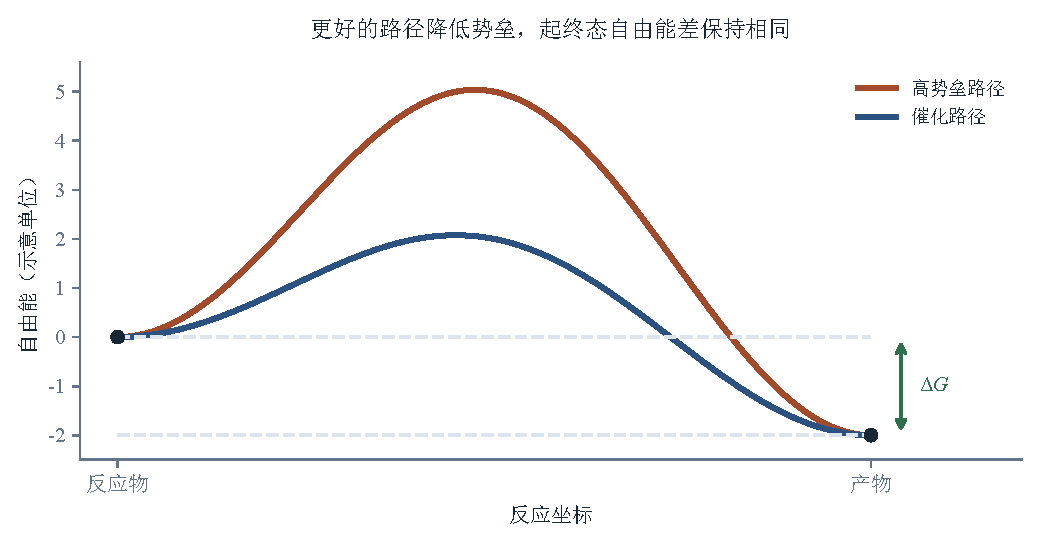
\includegraphics[width=\textwidth]{figures/activation-barrier.pdf}
\caption{催化改变路径与动力学势垒。图中的两条示意路径有相同起终态，$\Delta G$保持相同；降低活化自由能有助于加快速率，反应平衡由起终态决定。}
\label{fig:mechanism-activation-barrier}
\end{figure}
\subhead{智能在这条链上的位置}

智能可以筛选催化剂、寻找新反应路线、优化工艺窗口、调度能源并预测故障。催化会改变反应路径与速率，工艺整合也能回收热量、减少分离支出。改进应通过整个过程的能耗、良率、产能、安全与停机时间来衡量。

更麻烦的是，智能系统自身也在资源势垒之内。数据中心可以通过硬件、冷却和利用率提升显著改善能效，但“效率提高”不等于“物理基础消失”，大规模计算仍然要占用设备、土地、电力、冷却系统、技术链条和维护能力。\cite{masanet2020recalibrating}信息处理本身也不是脱离物理的幽灵，兰道尔原理至少提醒我们，信息擦除和逻辑不可逆操作存在热力学下限，尽管这一原理不能被粗暴地直接换算成所有现实计算系统的总能耗。\cite{landauer1961}

因此，判断一项技术是否真正降低现实代价，不能只看它在信息空间中生成了多少方案，而要看它是否减少了现实中的材料消耗、能量损耗、工艺步骤、维护负担和长期不可逆后果。如果一个方案只是把消耗转移到更深的技术链条、能源系统、算力后台或维护结构中，它没有突破资源势垒，只是改变了资源势垒的位置。真正可靠的技术进步，不是用比特逃离原子，而是在原子的硬约束中，用更好的路径完成不可豁免的状态转移，现实改变的本质，不是让可能性出现，而是让物质在可用能推动下，进入一个可维持的新秩序。

\subsection{宏观质量堆积与重力势能库的建立}

技术系统向物质底层推进时，遇到的边界形式取决于尺度。改动的对象越大、越小、越分散，阻挡它的东西就越不是同一类东西；上一段说的那三种边界因此会在不同的尺度上轮流成为主导项，而哪一项主导，决定了这一层的成本该往哪里记。

物质重构最常见的误判，是把原子世界想象成一种可以任意缩放、任意编辑、任意循环的软件空间。宏观上，似乎只要有更好的规划，就能改写城市和基础设施；微观上，似乎只要技术继续进步，就能无限缩小、无限精密；资源上，似乎只要回收体系足够完善，物质就可以被无限循环。现实并不是这样。原子世界有尺度，尺度一变，阻力的形态就会改变：宏观尺度上，阻力表现为质量、惯性和沉没结构；微观尺度上，阻力表现为热噪声、缺陷、量子效应和散热压力；元素尺度上，阻力表现为丰度、分布、提纯和循环不可逆。物质重构不是在一个均匀平面上移动符号，而是在不同尺度中穿过不同的物理边界，可以把它压缩为一句话：\key{宏观世界太重，微观世界太吵，元素世界太散。}

\subhead{质量与惯性}

先看宏观尺度，它的第一性约束是质量。质量不是单纯的重量，而是过去做功的沉积，凡是已经被开采、运输、抬升、固定、连接和维护的东西，都不只是物体，而是材料、能量、土地、劳动、制度和时间共同凝结成的结构，建筑、道路、桥梁、地铁、电网、管网、港口和厂房，都是过去投入在现实中的物理记忆。城市尤其如此，城市不是地图上的区域，也不是经济活动的抽象容器，而是亿万吨钢筋、水泥、玻璃、沥青、铜缆、管道和设备被抬升、固定、连接之后形成的高势能系统。建筑抵抗重力，桥梁跨越空间，地铁穿透地层，电网输送功率，管网维持流动，道路组织人和物的运动，城市是固化的能量，也是凝固的历史做功。

这类堆积的规模可以用物质流来衡量。水泥、钢铁、砂石等建筑材料构成了现代社会的物质存量主体，二十世纪全球社会经济物质存量增长了二十余倍，其中建筑和基础设施占绝大部分；\cite{krausmann2017global}人类每年搬运的土石方和沉积物总量已经与全球河流的自然输沙量相当甚至更高，在部分流域，人类搬运量超过自然侵蚀量。\cite{syvitski2005impact}城市就是这些流量的最终沉淀形式，这也正是原子世界更新缓慢的原因：旧建筑不是可以删除的文件，旧道路不是可以回滚的版本，旧管网不是可以重绘的图层，它们占据空间，绑定生活，牵连产权、金融、法规、习惯和日常路线。重构一片城区，不只是生成更好的方案，而是废弃已经固化的材料和势能，再支付拆除、运输、污染、替代、施工和社会协调成本。

到这里可以回答一个合理的反驳：如果质量是主要阻力，那么单位成本更低的方案应该自动胜出，为什么实际不是这样。原因是质量约束并不只体现在造价上，它通过产权、管网接口、施工窗口、生活习惯和既有路线把替换成本分散到很长时间里，单个决策者看到的往往只是其中一小段，于是更优方案在局部账面上划算，在整体账面上不划算。质量带来的这种性质有两面：一面是可靠，另一面是难改。桥梁之所以可用，是因为它足够坚固；城市之所以难改，也是因为它足够沉重。基础设施之所以能长期服务，是因为它把物质固定在稳定结构中；基础设施之所以难以快速迭代，也是因为这种稳定结构已经嵌入现实生活，宏观世界的阻力不是偶然阻力，而是过去成功建造所留下的惯性。

所以，许多技术落地不是败给观念保守，而是败给质量堆积：一个更优的交通方案，不能自动搬走旧道路；一个更好的能源系统，不能瞬间替换电网；一个更聪明的城市算法，不能让楼宇、管网、停车场、地铁线路和土地格局同步重排。宏观尺度的重构，本质上是在已经存在的重量中改写重量。这也是为什么数字技术进入原子世界时，常常先选择覆盖，而不是重建：给旧道路加导航，给旧工厂加传感器，给旧医院加AI分诊，给旧城市加监控平台，比推倒重构底层结构便宜得多。先覆盖而不是重建，不是偶然选择，而是宏观质量惯性下的现实路径：旧世界太重，新技术只能先附着在旧世界表面。

\subhead{重力势能库}

把建筑材料抬高，会增加重力势能。对给定质量与平均抬升高度，理想净功为

\begin{equation}
W=m\,g\,h
\end{equation}

$W$为重力势能增量，$m$为质量，$g$为当地重力加速度，$h$为平均抬升高度。以$m=10^8$千克、$h=250$米计算，$W$约为$2.45\times10^{11}$焦耳。设计能够改变用料、结构与高度；给定这些量，抬升账目才固定下来。施工中的耗散、材料制造与其他能耗另计。拆除释放的势能通常会耗散，能够回收多少取决于实际装置。城市更新还受拆解、运输、基础设施、产权与持续服务约束，储存的势能只占其中一项。

年度材料流显示另一种规模。2026年出版的USGS与worldsteel资料分别汇总2025年水泥与钢铁产量，前者在40亿吨量级，后者接近20亿吨。\cite{usgs2026cement,worldsteel2026figures} 水泥不等于熟料，理论反应热不等于全流程实际能耗，核算时须分别采用对应产量与工艺。矿山、加工、运输与施工共同构成一条持续运行的物质通道，城市是这条通道长期积累的结果。

势能库建成之后，它的约束方式与流量型能源不同。木材和畜力的约束是通量，只要当年产出不够，系统就停止扩张；固化质量的约束是存量，它不限制继续堆叠，却把改变的成本抬高到必须在很长时间里摊销。一座城市的重心、管网走向、道路格局和土地权属会同时约束此后几十年的所有改造方案，新的方案只能在既定几何中寻找缝隙。宏观尺度的阻力因此有一个反直觉的性质：它并不妨碍建造，它妨碍的是重新建造。

\subsection{微观尺度缩微的量子效应与热流密度极限}

把尺度缩小，情况并没有变简单。宏观尺度上，物体越大越难搬动；微观尺度上，结构越小越难控制，而且控制的对象从位置变成了概率。缩微在物理上从来不是简单的比例缩小，尺寸每下降一个量级，起作用的物理机制就会换一批。芯片是这条路径上被走得最远的一个例子，它同时也把缩微的两类极限暴露得最清楚：一类来自量子力学，一类来自热力学。

\subhead{噪声与热}

人们常以为小意味着轻，轻意味着便宜，但越接近原子、电子和量子尺度，世界越不再像宏观物体那样稳定可控，热噪声、表面效应、缺陷概率、量子隧穿、材料涨落、测量扰动和散热密度开始变得不可忽略。微观世界的阻力不是搬不动，而是控不稳；不是质量太大，而是扰动太多。芯片是最典型的例子：比特看似轻盈，软件看似可以无限复制，但制造比特的物理底座极其沉重。要让电子在纳米尺度按人类意图稳定运动，需要高纯材料、洁净室、真空环境、精密光刻、温度控制、化学处理、缺陷检测和全球供应链。芯片越小，制造它所需的环境控制系统越大；电子路径越短，支撑它的秩序密度要求越高，微观世界不是越轻越便宜，而是越精密越依赖庞大的后台工程。

微观缩小并不是简单比例缩小。宏观加工可以容忍粗糙，微观制造必须压低杂质、振动、热扰动和缺陷：一个肉眼不可见的颗粒，可能毁掉一片复杂结构；一个微小工艺漂移，可能影响大量器件性能；一个局部热点，可能限制整个系统的功率密度。越小的结构，越依赖更大的环境控制系统，小不是无重量，而是把重量转化为秩序密度。工程史给出了这条路径的终点：晶体管尺寸在几十年里持续缩小的时候，功耗密度还能按比例下降，频率可以不断提高，这一趋势在2005年前后停止，此后时钟频率长期停留在数吉赫兹量级，芯片性能的提升越来越依靠并行和专用结构，而不是继续提高单核频率。\cite{esmaeilzadeh2011dark}随之出现的问题是暗硅：受功率密度和散热能力限制，芯片上大部分晶体管在同一时刻无法同时以最高频率工作，一部分面积必须在任意时刻保持低功耗状态。\cite{esmaeilzadeh2011dark}

这条路径并没有被完全堵死，但绕开的办法只是把约束换了位置。三维堆叠、专用加速器和先进封装确实把一部分压力从尺寸转移出去，代价是散热通道变得更长、互连更复杂、良率更敏感，原来落在晶体管上的限制改由热流密度和封装工艺承担。这就是微观尺度的悖论：产品越轻，制造条件越重；单个元件越小，系统后台越大；信息越便宜，信息底座越昂贵。先进制造并不是物质性消失，而是物质性被压入更深的工艺、设备、能源和环境控制之中。

\subhead{量子效应：隧穿与统计涨落}

量子效应进入制造流程的方式，先是隧穿，然后是统计涨落。芯片上控制电流通断的栅极靠一层极薄的绝缘层隔开沟道，这层氧化物的厚度在持续缩微中降到了1.2到1.5纳米，也就是五六个原子层的量级。在这个厚度上，电子不再被势垒完全挡住，它有确定的概率直接穿过绝缘层，形成隧穿漏电流。漏电流随厚度指数上升，一旦它超过开关本身所需的电荷，继续减薄绝缘层就不再带来收益，只能改用高介电常数材料去换回等效的厚度。这是量子力学直接进入工艺决策的一个例子：不是工艺做不到更薄，而是更薄之后器件不再按电路设计的规则工作。

统计涨落来自同一个方向。器件沟道里参与导电的掺杂原子数目随体积缩小而下降，当数目降到几十个量级时，原子个数的随机波动直接转化为器件参数（如阈值电压）的器件间差异，同一批芯片上相邻的两个晶体管可能表现出明显不同的特性。这条约束无法靠提高加工精度消除，因为它的来源是掺杂原子的离散性和泊松统计，而不是机器的定位误差。类似的涨落还出现在制造工艺的上游：光刻使用的极紫外光波长13.5纳米，单个光子能量约92电子伏特，是深紫外光子的十多倍，在相同曝光剂量下到达晶圆的光子数目只有后者的十几分之一。光子到达服从泊松分布，落入一个小面积区域的光子数目的相对涨落随数目的平方根下降，特征尺寸缩小、区域面积减小时，光子数急剧下降，相对涨落急剧上升，本该平直的线条边缘因此变成锯齿状。要让涨落减半，曝光剂量必须提高到四倍。把这条统计关系写成式子是直接的，

\begin{equation}
\sigma_{N}=\sqrt{N},
\qquad
\frac{\sigma_{N}}{N}=\frac{1}{\sqrt{N}}
\end{equation}

式中 $N$ 为落入某一小面积区域的光子数，无量纲计数，也可以换成其他相互独立、随机到达的事件的计数；$\sigma_{N}$ 为它的标准差，量纲与 $N$ 相同；$\sigma_{N}/N$ 为相对涨落，无量纲。第二式说明相对涨落随计数按平方根下降：要让涨落减半，$N$ 必须增大到四倍。这正是特征尺寸缩小之后曝光剂量必须急剧上升的原因，也是极紫外光刻必须以二十千瓦级的激光输入换取二百五十瓦级曝光功率的原因之一。它的适用边界是：平方根关系只对相互独立、平均到达率稳定的泊松过程成立；若光源强度本身漂移，或者相邻区域的曝光存在关联，实际涨落会偏离 $1/\sqrt{N}$，所需剂量必须实测，不能按这个式子外推。为了在硅片上得到一条确定的线，上游必须投入远高于此的能量，量产极紫外光刻机的能量转换效率因此长期低于2\%：输入二十千瓦级的激光功率，最终可用于曝光的极紫外光只有二百五十瓦量级，其余都变成废热、碎片和动能冲击。\cite{debisschop2018stochastic}这里出现的不是工艺粗糙，而是确定性本身的代价：在原子尺度的加工区域里，每一次曝光只涉及有限个光子，统计规律就必然在成品上留下痕迹。

\subhead{热流密度墙}

热也是微观边界的一部分，计算、通信、制造和控制都要耗能，耗能就要散热，微观结构可以提高密度，却不能取消热流。器件越密集，功率越集中，散热越成为限制，很多时候限制系统继续前进的不是逻辑设计，而是热如何排出、噪声如何压低、缺陷如何控制。散热能力由材料导热、界面热阻和冷却介质共同决定，通道越窄，单位面积能带走的热流越难提高，风冷能够稳定处理的热流密度被限制在每平方厘米百瓦量级，超过这个水平就必须引入液冷、相变或更复杂的封装结构。把这个约束写成式子是直接的，

\begin{equation}
q=\frac{P}{A}=-k\,\frac{\Delta T}{L}
\end{equation}

$q$ 为热流密度，单位瓦每平方米，正文中风冷的上限用每平方厘米百瓦表示，合 $10^{6}$ 瓦每平方米量级；$P$ 为需要排出的功率，单位瓦；$A$ 为散热面积，单位平方米；$k$ 为材料的导热系数，单位瓦每米开尔文；$\Delta T$ 为沿散热路径的温差，单位开尔文；$L$ 为散热路径长度，单位米；负号表示热流方向沿着温度下降的方向。等号右边的三个量各有各的上限：$\Delta T$ 受器件工作温度与外部环境的夹逼，$k$ 由材料决定，$L$ 在三维堆叠中只会变长。通道变窄之后单位面积能带走的热流更难提高，对应的就是 $L$ 增大而 $q$ 下降；而功率密度的上升速度快于这几项的改善速度，差额就落在频率停滞和暗硅上。它的适用边界是：这是稳态、单一导热机制下的线性关系，相变、对流与辐射不遵从这一形式；真实封装中的界面热阻往往比材料本身更限制 $q$，所以这个式子给出的是量级判断，不是封装设计公式。功率密度的上升速度却比散热能力的改善快得多，两者之间的差额就表现为频率停滞和暗硅。

把这条约束放大到设施尺度，形状是一样的。数据中心把计算集中到少数几个地点，散热、供电和土地随之集中，冷却系统的规模成为选址与扩容的前置条件，能效改善可以把单位算力的能耗压下去，却压不掉热流本身。信息系统越往微观深入，它的上游越依赖一套宏大的宏观工程，而宏观工程的散热能力有上限。芯片越先进，这个上限越紧。\key{信息系统的尽头，仍然是热力学系统。}

\subsection{宇宙元素丰度与物质循环的热力学约束}

如果说宏观尺度的阻力来自质量，微观尺度的阻力来自噪声，那么元素尺度的阻力则来自丰度和分布。元素的多寡不由需求决定，而由核合成和行星分异决定，技术可以改变提取效率，不能改变分布本身。这一层的约束方式与前两层不同：质量可以被搬动，噪声可以被隔离，元素的分布只能被接受，然后靠更大的处理量、更长的流程和更高的能耗去迁就它。也正因为如此，元素层面的约束最难被工程手段绕过，最容易在供应紧张时以价格和工期的方式显形。

\subhead{丰度与熵税}

元素不是均匀摆放在地球表面的材料库，它们来自宇宙核合成、行星形成、地质分异、矿化过程和漫长地球历史，碳、氧、硅、铁、铝、铜、锂、镍、钴、稀土、铂族元素，并不是以人类需要的方式均匀存在。宇宙中有某种元素，不等于地球上有足够可用储量；地壳中存在，不等于形成了可开采矿床；产品中含有，不等于能够低成本回收。地壳的元素分布本身就是高度不均匀的：氧和硅两种元素合计约占地壳质量的四分之三，铝和铁各占百分之几，而铜的平均丰度在百万分之六十量级，锂在百万分之二十量级，稀土元素合计在百万分之一百至两百量级，铂族元素则低到十亿分之一量级。\cite{rudnick2003composition}这些比例由恒星核合成和行星分异过程决定，不受需求影响，技术可以提高提取效率，可以寻找替代材料，但不能让某种元素在世界上变得更常见。

由此推出的判断与上两节一致：资源问题的关键，不是“有没有某种元素”，而是它是否以足够浓度、足够规模、足够稳定、足够低成本的方式处在可用状态中。低品位矿不是没有资源，而是资源过于分散，需要更高能耗和更大处理量才能利用；稀有元素也不是完全不存在，而是浓度低、分布不均、提取复杂、伴生关系强，并常常受到地理和产业链约束。这使得物质循环不可能成为热力学意义上的免费过程：回收不是把物质重新拿回来这么简单，而是把已经分散、混合、污染、降级和嵌入复杂产品中的物质重新带回可用状态，它需要收集、拆解、分离、提纯、再加工和质量控制。循环可以降低原生开采压力，但循环本身也消耗能量、设备和时间。

回收需要收集、拆解、分离与再加工。这些步骤消耗资源，也可能比原生开采与冶炼节约大量能量。要比较的是同一材料、同等品质与同一边界下的全流程：产品中的浓度、污染、拆解设计与运输距离，都可能改变结果。循环的价值来自实际减少的新开采、能耗与废弃负担。

这可以称为元素层面的熵税。只要物质被分散、混合、污染和降级，重新集中它、分离它、提纯它，就必须付出新的能量、设备和时间，技术可以降低这笔税，不能让这笔税归零。分散的物质不会免费回到高浓度状态，混合的材料不会免费拆分成纯净组分，循环本身不是逃离熵增，而是在熵增之后重新支付秩序恢复成本。因此，元素尺度提醒我们：物质世界不是无限可调的库存，而是由丰度、位置、浓度、化学状态和循环损耗共同构成的约束场。技术可以提高提取效率，改善替代材料，优化回收流程，但不能让宇宙元素丰度重新洗牌，不能让分散物质无成本集中，不能让混合物无能耗分离，不能让循环没有熵税。

\subhead{元素从哪里来}

元素供给带着宇宙与地质历史。大爆炸核合成主要形成氢、氦，恒星内部反应与后续演化产生许多更重元素。铁峰附近之后的合成包含恒星中的慢中子俘获，以及中子星并合等环境中的快中子俘获等路线。\cite{steigman2007primordial,kobayashi2020origin} 地球上的可用矿床还要经过行星分异、岩浆、热液与风化富集。工程面对的是这些过程留下的浓度、位置与化学状态。

行星形成和地质分异又对这份清单做了一次重新分配。地球形成时的分异过程把亲铁元素带进地核，把亲石元素留在幔壳，地壳中的可用矿床再经过数十亿年的岩浆活动、热液迁移和风化富集才形成。这意味着两件事：一是元素的绝对数量由宇宙和行星过程给定，二是这些元素在地表是否集中成矿，取决于后来的地质历史。人类可以开采的部分，只是这两个过程叠加之后留下的少数异常富集区。技术能改变的是对富集区的要求，品位可以从百分之几降到百万分之几，但每降一个量级，处理量、能耗和废物就要上一个台阶，熵税的斜率不会变。把处理量与品位之间的关系写成式子是直接的，

\begin{equation}
M=\frac{m}{\theta}
\end{equation}

这里 $M$ 为获取给定目标元素所必须处理的原矿质量，单位千克或吨；$m$ 为其中目标元素的质量，单位与 $M$ 相同；$\theta$ 为品位，即目标元素在原矿中所占的质量分数，无量纲，工业上常用百分比或百万分之一表示。反比关系给出那句判断的全部内容：品位每下降一个数量级，为了得到同样多的目标元素，需要开采、破碎、浸出和处理的物料就上升一个数量级，能耗、试剂与废物同步上升，熵税的斜率就是这条反比关系。它的边界有两处：一是这里只算物料量，不含提取率，实际回采与选冶的回收率都小于 1，真实处理量比 $M$ 更大；二是当矿物相复杂、多元素伴生时，能耗随品位下降常常比 $1/\theta$ 更快，因为磨矿要更细、分离步骤要更多。因此在真实矿山上，这个式子是乐观下限，不是预测。

\subhead{三种尺度的共同含义}

把三个尺度放在一起，它们共同说明：原子世界不能像软件一样任意重写。宏观上，质量留下惯性；微观上，噪声限制控制；元素层面，丰度和分布约束可用性。每一层都有自己的边界，每一层都要求不同形式的代价，物质重构不是一场在抽象空间中的优化，而是在不同尺度上制造和维持结构的过程。这也意味着，物质重构的难点不只是“能不能设计出来”：设计发生在表示空间，尺度边界发生在现实空间，一个更好的城市规划必须穿过宏观质量惯性，一个更先进的芯片设计必须穿过微观制造极限，一个更理想的能源方案必须穿过元素丰度、矿产分布和循环热力学。方案可以轻盈，尺度不会轻盈。

三个尺度上的边界形态不同，指向的却是同一件事：物质重构必须在尺度中发生。它可以优化城市更新路径，减少拆除浪费；可以改进芯片设计和制造控制，降低缺陷率；可以寻找替代材料，提高资源循环效率；可以在复杂供应链中减少无效消耗。这些都做得到，但穿越尺度边界时的浪费减少了，尺度边界本身不会消失。尺度边界的意义，不是说技术无法进步，而是提醒我们技术进步必须在尺度中发生，真正成熟的物质重构，不是幻想把世界压成可编辑的平面，而是理解不同尺度上的阻力形态：在宏观上尊重惯性，在微观上管理噪声，在元素层面承认可用性的稀缺。原子世界不是慢版软件，它有重量，有热，有噪声，有丰度，有历史，它的更新缓慢，不只是因为人类组织低效，而是因为物质本身在不同尺度上保留了自身的抵抗。\key{世界可以被改变，但不能被任意改写。}

以上三种边界都是关于空间和物质的：多大的质量被固定，多小的结构被维持，多稀的元素被集中。它们回答的是物质在尺度上如何抵抗重构，没有回答时间被压缩时会发生什么。而时间压缩不会改变这些边界，只会把它们重新组织一遍：同样多的质量、同样多的热、同样多的缺陷，被要求在同一条更短的窗口里通过系统。通量一旦成为主要约束，尺度上的三重边界就会以另一种形式重新出现。

% <<<<<<<<<< parts/book-ch02a.tex <<<<<<<<<<


% >>>>>>>>>> parts/book-ch02b.tex >>>>>>>>>>
